\documentclass[journal,12pt,twocolumn]{IEEEtran}

\usepackage{setspace}
\usepackage{gensymb}
\singlespacing
\usepackage[cmex10]{amsmath}

\usepackage{amsthm}

\usepackage{mathrsfs}
\usepackage{txfonts}
\usepackage{stfloats}
\usepackage{bm}
\usepackage{cite}
\usepackage{cases}
\usepackage{subfig}

\usepackage{longtable}
\usepackage{multirow}

\usepackage{enumitem}
\usepackage{mathtools}
\usepackage{steinmetz}
\usepackage{tikz}
\usepackage{circuitikz}
\usepackage{verbatim}
\usepackage{tfrupee}
\usepackage[breaklinks=true]{hyperref}
\usepackage{graphicx}
\usepackage{tkz-euclide}

\usetikzlibrary{calc,math}
\usepackage{listings}
    \usepackage{color}                                            %%
    \usepackage{array}                                            %%
    \usepackage{longtable}                                        %%
    \usepackage{calc}                                             %%
    \usepackage{multirow}                                         %%
    \usepackage{hhline}                                           %%
    \usepackage{ifthen}                                           %%
    \usepackage{lscape}     
\usepackage{multicol}
\usepackage{chngcntr}

\DeclareMathOperator*{\Res}{Res}

\renewcommand\thesection{\arabic{section}}
\renewcommand\thesubsection{\thesection.\arabic{subsection}}
\renewcommand\thesubsubsection{\thesubsection.\arabic{subsubsection}}

\renewcommand\thesectiondis{\arabic{section}}
\renewcommand\thesubsectiondis{\thesectiondis.\arabic{subsection}}
\renewcommand\thesubsubsectiondis{\thesubsectiondis.\arabic{subsubsection}}


\hyphenation{op-tical net-works semi-conduc-tor}
\def\inputGnumericTable{}                                 %%

\lstset{
%language=C,
frame=single, 
breaklines=true,
columns=fullflexible
}
\begin{document}

\newcommand{\BEQA}{\begin{eqnarray}}
\newcommand{\EEQA}{\end{eqnarray}}
\newcommand{\define}{\stackrel{\triangle}{=}}
\bibliographystyle{IEEEtran}
\raggedbottom
\setlength{\parindent}{0pt}
\providecommand{\mbf}{\mathbf}
\providecommand{\pr}[1]{\ensuremath{\Pr\left(#1\right)}}
\providecommand{\qfunc}[1]{\ensuremath{Q\left(#1\right)}}
\providecommand{\sbrak}[1]{\ensuremath{{}\left[#1\right]}}
\providecommand{\lsbrak}[1]{\ensuremath{{}\left[#1\right.}}
\providecommand{\rsbrak}[1]{\ensuremath{{}\left.#1\right]}}
\providecommand{\brak}[1]{\ensuremath{\left(#1\right)}}
\providecommand{\lbrak}[1]{\ensuremath{\left(#1\right.}}
\providecommand{\rbrak}[1]{\ensuremath{\left.#1\right)}}
\providecommand{\cbrak}[1]{\ensuremath{\left\{#1\right\}}}
\providecommand{\lcbrak}[1]{\ensuremath{\left\{#1\right.}}
\providecommand{\rcbrak}[1]{\ensuremath{\left.#1\right\}}}
\theoremstyle{remark}
\newtheorem{rem}{Remark}
\newcommand{\sgn}{\mathop{\mathrm{sgn}}}
\providecommand{\abs}[1]{\vert#1\vert}
\providecommand{\res}[1]{\Res\displaylimits_{#1}} 
\providecommand{\norm}[1]{\lVert#1\rVert}
%\providecommand{\norm}[1]{\lVert#1\rVert}
\providecommand{\mtx}[1]{\mathbf{#1}}
\providecommand{\mean}[1]{E[ #1 ]}
\providecommand{\fourier}{\overset{\mathcal{F}}{ \rightleftharpoons}}
%\providecommand{\hilbert}{\overset{\mathcal{H}}{ \rightleftharpoons}}
\providecommand{\system}{\overset{\mathcal{H}}{ \longleftrightarrow}}
	%\newcommand{\solution}[2]{\textbf{Solution:}{#1}}
\newcommand{\solution}{\noindent \textbf{Solution: }}
\newcommand{\cosec}{\,\text{cosec}\,}
\providecommand{\dec}[2]{\ensuremath{\overset{#1}{\underset{#2}{\gtrless}}}}
\newcommand{\myvec}[1]{\ensuremath{\begin{pmatrix}#1\end{pmatrix}}}
\newcommand{\mydet}[1]{\ensuremath{\begin{vmatrix}#1\end{vmatrix}}}
\numberwithin{equation}{subsection}
\makeatletter
\@addtoreset{figure}{problem}
\makeatother
\let\StandardTheFigure\thefigure
\let\vec\mathbf
\renewcommand{\thefigure}{\theproblem}
\def\putbox#1#2#3{\makebox[0in][l]{\makebox[#1][l]{}\raisebox{\baselineskip}[0in][0in]{\raisebox{#2}[0in][0in]{#3}}}}
     \def\rightbox#1{\makebox[0in][r]{#1}}
     \def\centbox#1{\makebox[0in]{#1}}
     \def\topbox#1{\raisebox{-\baselineskip}[0in][0in]{#1}}
     \def\midbox#1{\raisebox{-0.5\baselineskip}[0in][0in]{#1}}
\vspace{3cm}
\title{\textbf{AI 1103 - Assignment 1}}
\author{T. Rohan \\ CS20BTECH11064}
\maketitle
\newpage
\bigskip
\renewcommand{\thefigure}{\theenumi}
\renewcommand{\thetable}{\theenumi}
Download all python codes from 
\begin{lstlisting}
https://github.com/rohanthota/Assignment_1/codes/Assignment_1.py
\end{lstlisting}
%
and latex codes from
%
\begin{lstlisting}
https://github.com/rohanthota/Assignment_1/Assignment 1.tex
\end{lstlisting}
\section * {\emph{Question}}
A class has 15 students whose ages are 14, 17, 15, 14, 21, 17, 19, 20, 16, 18, 20, 17, 16, 19 and 20 years. One student is selected in such a manner that each has the same chance of being chosen and the age X of the selected student is recorded. What is the  probability distribution of the random variable X ? Find the  mean, variance and standard deviation of X.

\section*{\emph{Solution}}
There are a total of 15 students in the class, each equally likely to be selected.
\\Hence, we could say that the probability of each student to be chosen is \textbf{$\frac{1}{15}$}.

   Number of students of age \textbf{14} = \emph{2}
\\ Number of students of age \textbf{15} = \emph{1}
\\ Number of students of age \textbf{16} = \emph{2}
\\ Number of students of age \textbf{17} = \emph{3}
\\ Number of students of age \textbf{18} = \emph{1}
\\ Number of students of age \textbf{19} = \emph{2}
\\ Number of students of age \textbf{20} = \emph{3}
\\ Number of students of age \textbf{21} = \emph{1}

We are assigning 
\\  \textbf{X=0} for the case when a student of age \textbf{14} is picked,
\\  \textbf{X=1} for the case when a student of age \textbf{15} is picked, 
\\  \textbf{X=2} for the case when a student of age \textbf{16} is picked,
\\  \textbf{X=3} for the case when a student of age \textbf{17} is picked,
\\  \textbf{X=4} for the case when a student of age \textbf{18} is picked,
\\  \textbf{X=5} for the case when a student of age \textbf{19} is picked,
\\  \textbf{X=6} for the case when a student of age \textbf{20} is picked,
\\  \textbf{X=7} for the case when a student of age \textbf{21} is picked,


Since we know that probability of an outcome to happen is \textbf{P(outcome) = $\frac{\textit{No. of favourable outcomes}} {\textit{Total No. of outcomes}}$}
Therefore, 
\begin{align*}
    P(\textbf{X=0}) = \frac {2}{15} = 0.13333334
   \\ P(\textbf{X=1}) = \frac {1}{15} = 0.06666667
   \\ P(\textbf{X=2}) = \frac {2}{15} = 0.13333334
   \\ P(\textbf{X=3}) = \frac {3}{15} = 0.20000000
   \\P(\textbf{X=4}) = \frac {1}{15} = 0.06666667
   \\ P(\textbf{X=5}) = \frac {2}{15} = 0.13333334
   \\ P(\textbf{X=6}) = \frac {3}{15} = 0.20000000
   \\ P(\textbf{X=7}) = \frac {1}{15} = 0.06666667
\end{align*}

Therefore, the p
\begin{center}
\begin{tabular}{|c|c|c|c|c|c|c|c|c|}
\hline
\textbf{X} & 0 & 1 & 2 & 3 & 4 & 5 & 6 & 7 \\
\hline
\textbf{P(X)} & $\frac {2}{15}$ & $\frac {1}{15}$ & $\frac {2}{15}$ & $\frac {3}{15}$ & $\frac {1}{15}$ & $\frac {2}{15}$ & $\frac {3}{15}$ & $\frac {1}{15}$ \\
\hline 
\end{tabular}
\end{center}


\begin{enumerate}
    
\item The mean E(X) of the distribution is given by E(X) = $\Sigma^n_{i=1}$ $x_i$ $P_i$ 
\begin{align*}
    
    $  =  14 * \frac{2}{15} + 15 * \frac{1}{15} + 16 * \frac{2}{15} + 17 * \frac{3}{15} + 18 * \frac{1}{15} + 19 * \frac{2}{15} + 20 * \frac{3}{15} + 21 * \frac{1}{15}$
    \\\\$=\frac{28+15+32+51+18+38+60+21}{15}$
    \\\\$=\frac{263}{15}$
    
    
    \\\\Therefore \textbf{E(X) = 17.53}
\end{align*}
\item The variance of X is given by \textbf{Var(X) =  E($X^2$) - $[E(X)]^2$.}
\\ Here E($X^2$) is given by 
\begin{align*}
   
    E($X^2$) = $\Sigma^n_{i=1}$ $x^2_i$ $P_i$ 
    \\\\ $  =  14^2 * \frac{2}{15} + 15^2 * \frac{1}{15} + 16^2 * \frac{2}{15} + 17^2 * \frac{3}{15} + 18^2 * \frac{1}{15} + 19^2 * \frac{2}{15} + 20^2 * \frac{3}{15} + 21^2 * \frac{1}{15}$
    \\\\$=\frac{392+225+512+867+324+722+1200+441}{15}$
    \\\\$=\frac{4683}{15}$
    \\\\ Hence, Var (X) = $\frac{4683}{15}$ - $(\frac{263}{15})^2$
    \\\\ Var (X) = $\frac{4683}{15}$ - $\frac{69169}{225}$
    \\\\ Therefore \textbf{Var (X) = 4.78}
\end{align*}
\item Standard deviation is given by $\sigma_x$ = $\sqrt{Var(X)}$
\begin{align*}
     
     $\sigma_x$ = $\sqrt{4.78}$
     \\Hence, \textbf{Standard Deviation, $\sigma_x$ = 2.18}
\end{align*}
\hline
\\\\\\Drawing the comparison graph with ages on x-axis, probabilities on y-axis, blue bar representing simulations and orange bar representing theoretical value, we get
\\\\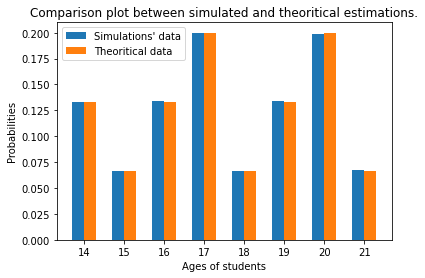
\includegraphics{Assignment 1 graph}
\end{enumerate}
\end{document}